\documentclass[12pt,a4paper]{report}
% \textheight = 30cm
% \voffset = -36pt
\footskip = 0cm

\usepackage{cmap}
\usepackage{type1ec}
\usepackage[T2A]{fontenc}
\usepackage[utf8]{inputenc}
\usepackage[russian]{babel}

\usepackage{amsmath,amstext,amssymb,amsthm}
\usepackage{fullpage}

\usepackage{ifpdf}
\ifpdf
  \usepackage[pdftex]{graphicx}
  \usepackage[pdftex,unicode,bookmarks=false]{hyperref}

  \pdfminorversion=5
  \pdfcompresslevel=9
  \pdfobjcompresslevel=9
\fi

\pagestyle{empty}

\graphicspath{{./figures/}}

\DeclareMathOperator{\EX}{\mathbb{E}}

\renewcommand{\thesection}{\arabic{section}}
\renewcommand{\thesubsection}{}

% Константа
\def\const{\mathop{\mathrm{const}}\nolimits}

% Модуль
\providecommand{\abs}[1]{\left\lvert{#1}\right\rvert}


\newtheorem*{definition}{Определение}
\newtheorem*{example}{Пример}
\newtheorem*{property}{Свойство}

\begin{document}

% --------------------------------------------------------------------------------------

\section{Administrivia}

В прошлом году лекции и семинары практически не отличались, в этом попробуем решать больше задач на семинарах.

\subsection*{Оценка}

$$
G_{final} = 0.3 \cdot G_{hw} + 0.3 \cdot G_{test} + 0.4 \cdot G_{exam}
$$

Домашние задания -- после семинаров. Контрольная -- между модулями.

\subsection*{План}

1-й модуль:

\begin{itemize}
  \item Анализ сложности алгоритмов
  \item Алгоритмы сортировки
  \item Структуры данных: списки, деревья, хэш-таблицы, кучи, системы непересекающихся множеств
\end{itemize}

2-й модуль:

\begin{itemize}
  \item Жадное программирование. Динамическое программирование.
  \item Алгоритмы на графах.
  \item Алгоритмы на строках.
  \item Что-нибудь специфичное для лингвистики/численных методов/баз данных
\end{itemize}

\subsection*{Литература}

\begin{enumerate}
  \item {\bf T.~Cormen et al. {\em Introduction to Algorithms}}
  \item Steven Skiena {\em The Algorithm Design Manual}
  \item Бабенко М.А.,~Левин М.В. {\em Введение в теорию алгоритмов и структур данных}
\end{enumerate}

% --------------------------------------------------------------------------------------

\section{Алгоритмы}

{\em Алгоритм} -- в очень узком смысле -- спецификация решения задачи с помощью компьютера, подразумевающей преобразование входных данных в выходные. Строгость такой спецификации должна быть достаточной для создания компьютерной программы (реализации алгоритма), решающей эту задачу.

Подавляющая часть описываемых в курсе алгоритмов уже имеет свои реализации в стандартных и сторонних библиотеках языков программирования. Хотелось бы просто использовать их, не изучая стоящих за ними алгоритмов, но
\begin{itemize}
  \item абстракции протекают: эффективное использование библиотечных функций часто требует понимания работы и сложности реализованных алгоритмов (hashing trick, sparce matrix, graphs, индексы в базах данных, ...);
  \item иногда требуется реализовать новый алгоритм или структуру данных в условиях, с которыми ещё никто не сталкивался;
  \item подробнее -- в повести {\em Профессия} Айзека Азимова.
\end{itemize}

Термины и действия, в которых описывается алгоритм, зависят от выбранной модели вычислений.
Фактически -- некоторое абстрактное описание того, как именно работает компьютер, для которого предназначен алгоритм.

% --------------------------------------------------------------------------------------

\section{Word RAM model}

Модель аппроксимирует устройство всех современных компьютеров с достаточной для наших целей точностью.

\begin{itemize}
  \item Память: 
  \begin{itemize}
    \item Составлена из элементарных двоичных элементов памяти -- битов. Биты объединены в ячейки ({\em слова}) ширины $w$. Каждая ячейка имеет {\em адрес} -- число от $0$ до $M-1$.
    \item В реальных процессорах значений $w$ несколько -- 8/16/32/64 бит. Отсюда размеры числовых типов в языках программирования.
    \item {\em Байт}, по определению -- минимальная адресуемая ячейка памяти.
    \item Если нужно представить число большее чем $2^w-1$, используем несколько ячеек.
    \item {\em Массив} -- конечное число последовательно расположенных ячеек памяти
    \item {\em Строка} -- массив чисел, соответствующих буквам согласно кодировке (ASCII, UTF-8, ...)
  \end{itemize}
  \item CPU: 
  \begin{itemize}
    \item Фиксированное число {\em регистров} $\{r_i\}$ -- встроенных неадресуемых ячеек памяти размера $w$ каждая.
    \item Исполняет {\em программу} -- список пронумерованных (элементарных) операций:
    \begin{itemize}
      \item {\tt load RAM[rx] -> ry}\\
          загрузить значение ячейки по адресу $r_x$ в регистр $r_y$
      \item {\tt store ry -> RAM[rx]}\\
            записать значение из регистра $r_y$ в память по адресу $r_x$\\
            кстати, отсюда же следует что $M \leq 2^w$
      \item {\tt add r1, r2 -> r3}\\
          сложить числа в регистрах $r_1$ и $r_2$, записать результат в $r_3$
      \item {\tt sub r1, r2 -> r3}
      \item {\tt mul r1, r2 -> r3, r4}
      \item {\tt div r1, r2 -> r3, r4}
      \item {\em побитовые логические операции, сдвиги, операции над числами с плавающей точкой, и любые другие процессорозависимые операции, если мы хотим добавить их в модель}
      \item {\tt jcmp r1, r2 -> L}\\
          переходит к операции под меткой $L$ если $r_1 < r_2$,
    \end{itemize}
    \item Каждая операция исполняются {\em за единицу времени}.
  \end{itemize}
\end{itemize}

\begin{verbatim}
Python:

A[i] = A[i-1] + 3
------------------------------------------------------------
                     Assembler:

t = A[i-1]           load RAM[rX] -> r1      # i
                     sub r1, 1 -> r1         # i-1
                     load RAM[A+r1] -> r2    # A[i-1]
A[i] = t + 3         add r2, 3 -> r3         # t + 3
                     add r2, 1 -> r4         # i = (i-1) + 1
                     stort r3 -> RAM[A+r4]   # A[i] = t + 3
\end{verbatim}

Очень грубо предположим:
\begin{itemize}
\item в языках программирования операциям над целыми числами $\leq (2^{64}-1)$ соответствует не более чем $K=\const$ элементарных операций;
\item элементарные операции выполняются не более чем за $t_0=\const$ времени.
\end{itemize}


\section{Временная сложность алгоритма}

Здесь и далее буква $t$ обозначает абсолютное время работы алгоритма:
$$
t(I, K, t_0)
$$
где $I$ -- некоторые входные данные.

Это -- функция, т.к. у детерменированного алгоритма для одних и тех же данных на одном том же компьютере время работы должно быть одинаковым.

\subsection*{Размер данных}

Практичнее оценивать время не на конкретных данных, а не данных некоторого размера $n$ (количество элементов массива, размерность матрицы, количество вершин и рёбер графа, разрядность входного числа, и т.~п.)
$$
t^*(n, K, t_0)
$$

Но $t^*$ не функция -- она может давать разные значения на одних и тех же параметрах. Например, сортировка массивов размера $n$ может сильно отличаться по времени в зависимости от начального расположения элементов. Необходимо как-то аггрегировать все возможные данные размера $n$: 

\begin{itemize}
\item {\em сложность в худшем случае} ({\em worst-case complexity}):
$$
\boxed{
  t_w(n, K, t_0) = \max_{I \in I_n}~{t(I, K, t_0)}  
}
$$
чаще всего мы будем работать именно с ней.
\item {\em ожидаемая сложность} (или сложность в среднем, если брать равномерное распределение входных данных)
$$
t_e(n, K, t_0) = \mathbb{E}_{I \in I_n} \left[ {t(I, K, t_0)} \right]
$$
\end{itemize}

\subsection*{Избавление от констант}

Нам часто важнее знать, как время работы алгоритма зависит от $n$, чем абсолютные значения $t$ и входящие в неё константы: 
\begin{itemize}
\item Константы $K$ и $t_0$ можно <<тривиально>> уменьшить выбрав более быстрый компьютер и/или низкоуровневый язык программирования;
\item при этом изменение констант даёт изменение времени исполнения не более чем в константное число раз;
\item $n$ обычно нельзя контролировать; в долгосрочной перспективе $n$ всегда растёт. 
\end{itemize}

Для таких оценок используется {\em асимптотический анализ}.

\section{Асимптотический анализ}

\subsection*{Оценка сверху}


\begin{figure}[!ht]
\centering
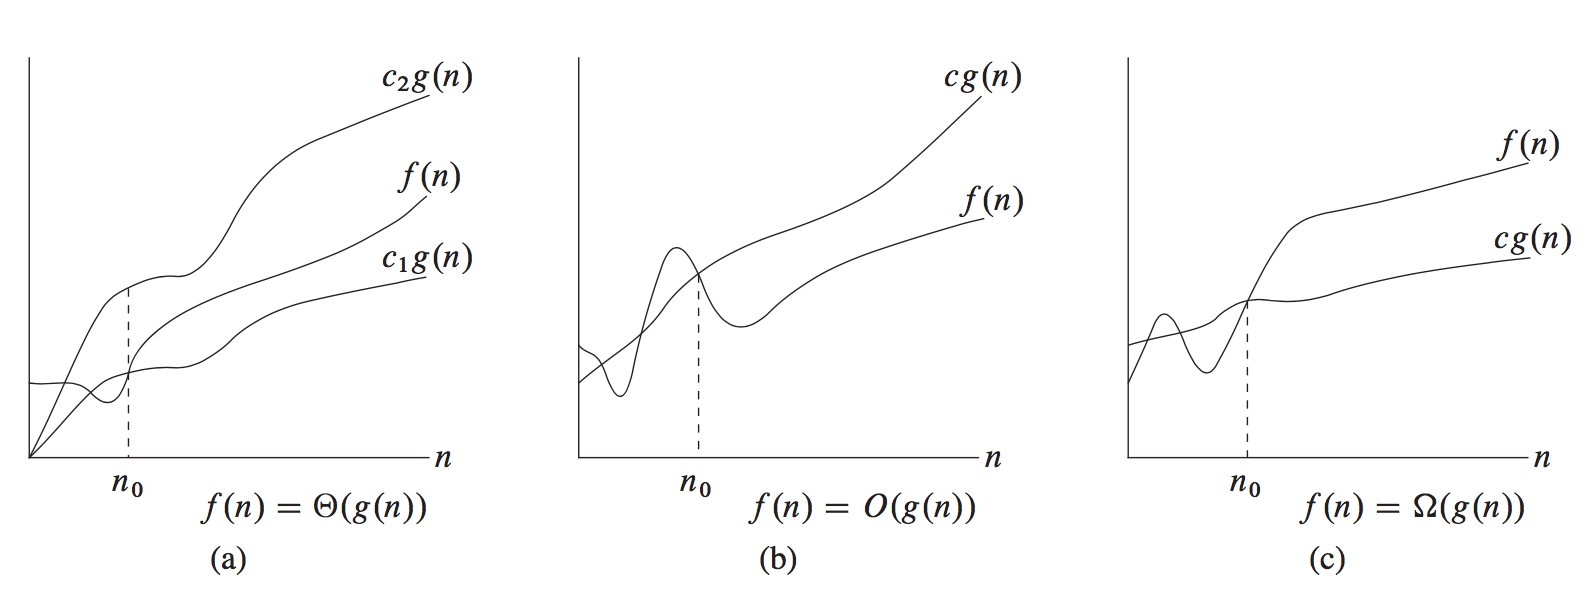
\includegraphics[width=17cm]{classes.png}
\end{figure}

\begin{definition}
Говорят, что $f(n)$ принадлежит классу функций $O(g(n))$, и пишут $f(n)=O(g(n))$, если
$$
\exists c>0, n_0>0:~ \forall n > n_0 ~~\to~~ 0 \leqslant f(n) \leqslant c \cdot g(n)
$$

\end{definition}

Иначе говоря, $t(n)=O(T(n))$, то $T(n)$ является оценкой $t(n)$ сверху при достаточно больших $n$ с точностью до постоянного множителя.


% ---------------------------------------------------------

\begin{example}
При оценке функции через O игнорируются константные множители:
$$
f(n) > 0,~ K=\const>0: ~~~~ K \cdot f(n) = O(f(n))
$$
\begin{proof}По определению: $n_0=1$, $c=K+1$\end{proof}
\end{example}

% ---------------------------------------------------------

\begin{example}
$$
f_1(n) = O(g_1(n)),~ f_2(n) = O(g_2(n)) ~~\Rightarrow~~ f_1(n) + f_2(n) = O(\max\{f_1(n), f_2(n)\})
$$
\end{example}

% ---------------------------------------------------------

\begin{example}
Члены низшего порядка также игнорируются:
$$
\frac{1}{2}n^2 - 3n = O(n^2)
$$
\begin{proof}По определению, нужно найти такое $c$ и $n_0$ чтобы
$$
\begin{gathered}
\frac{1}{2}n^2 - 3n \leqslant c n^2,~~~ n>n_0\\
\frac{1}{2} - \frac{3}{n} \leqslant c,~~~ n>n_0\\
\end{gathered}
$$
Выполняется при $n>0$ и $c \geqslant 1/2$
\end{proof}
\end{example}

% ---------------------------------------------------------

\begin{example}
В более общем случае:
$$
  \begin{gathered}
  f(n) = an^2 + bn + c,~~ a > 0\\
  f(n)=O(n^2)
  \end{gathered}
$$

\begin{proof}
Докажем, что найдутся такие $C$ и $n_0$, что
$$
  \begin{gathered}
  an^2 + bn + c \leqslant C n^2,~~~n>n_0\\
  a + \frac{b}{n}  + \frac{c}{n^2} \leqslant C
  \end{gathered}
$$

Пусть $n_0 = 2 \cdot \max\{\abs{b}/a, \sqrt{\abs{c}/a}\}$. Тогда
$$
  \begin{gathered}
    \frac{b}{n_0} = \begin{cases}
    = \frac{1}{2} a, & \abs{b}/a > \sqrt{\abs{c}/a}\ \\
    < \frac{1}{2} a, & \abs{b}/a < \sqrt{\abs{c}/a}\ \\
    \end{cases} \\
    \frac{c}{n^2_0} = \begin{cases}
    = \frac{1}{4} a, & \abs{b}/a < \sqrt{\abs{c}/a}\ \\
    < \frac{1}{4} a, & \abs{b}/a > \sqrt{\abs{c}/a}\ \\
    \end{cases}
  \end{gathered}
$$

$$
a + \frac{b}{n}  + \frac{c}{n^2}  \leqslant a + \frac{1}{2} a + \frac{1}{4} a \leqslant \boxed{\frac{7}{4} a = C}
$$
\end{proof}
\end{example}

% ---------------------------------------------------------

\begin{property}
$$
\boxed{
  \exists \lim_{n\to\infty} \frac{f(n)}{g(n)} = C \geqslant 0   ~~~\Rightarrow~~~   f(n) = O(g(n))
}
$$
\end{property}

% ---------------------------------------------------------

Обратите внимание: свойство работает только в одну сторону. Например, $n^2\cos n = O(n^2)$, но предел их отношения не существует.

\begin{figure}[!ht]
\centering
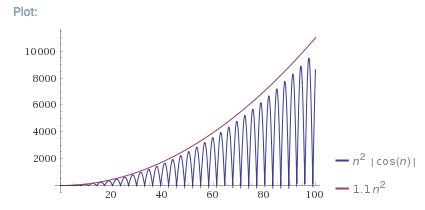
\includegraphics{cos.png}
\end{figure}

\subsection*{Оценка снизу}

$$
\Omega(g(n)) = \{f(n) : \exists c>0, n_0>0:~~ \forall n > n_0 ~~\to~~ 0 \leqslant c \cdot g(n) \leqslant f(n)\}
$$

\begin{property}
$$
f(n) = \Omega(g(n))   ~~\Leftrightarrow~~  g(n) = O(f(n))
$$
\end{property}


\subsection*{Точная оценка}

Для $O$ или $\Omega$, согласно определениям, верны нестрогие оценки: $2n = O(n^2)$ или $100n^3 = \Omega(n)$. С практической точки зрения они не очень информативны.

\begin{definition}
$$
  \begin{gathered}
  \Theta(g(n)) = \{f(n) : \exists c_1>0, c_2>0, n_0>0:~~ \forall n > n_0 ~\to~\\
  0 \leqslant c_1 \cdot g(n) \leqslant f(n) \leqslant c_2 \cdot g(n)\} \\
  \end{gathered}
$$
\end{definition}

\begin{definition}[альтернативное]
$$
  f(n) = \Theta(g(n)) ~~\Leftrightarrow~~  f(n) = O(g(n)) ~~\vee~~ f(n) = \Omega(g(n))
$$
\end{definition}

Иначе говоря, $f(n)=\Theta(g(n))$ означает что $g(n)$ ограничивает $f(n)$ сверху и снизу при достаточно больших $n$ с точностью до постоянного множителя.

Принадлежность к $\Theta$ также удобно вычислять через предел:
$$
\begin{gathered}
\lim_{n\to\infty} \frac{f(n)}{g(n)} = C > 0   ~~~\Rightarrow~~~   f(n) = \Theta(g(n))
\end{gathered}
$$

\newpage

\section{Пример: сортировка вставками}

\begin{verbatim}
def insertion_sort(A):
    for j in range(1, len(A)):
        # В этой точке отсортированый префикс в массиве
        # имеет длину j
        key = A[j]
        i = j
        while i>0 and A[i-1]>key:
            A[i] = A[i-1]
            i -= 1
        A[i] = key
    return A
\end{verbatim}




\subsection*{Итог}

Время работы и потребление памяти не оценивается в абсолютных единицах, поскольку они могут варьироваться в зависимости от языка программирования, компьютера и многих деталей реализации. Вместо этого ресурсы оцениваются асимптотическими классами, которые можно сранивать не оглядываясь на конкретные реализации.



\end{document}